\chapter{Segunda Iteración: Versión final e Integración}
\label{it2}

Como se explica en el la subsección \ref{metodologiadedesarrollo}, en la que se expone la metodología de desarrollo utilizada para el proyecto, este sufre de tres grandes iteraciones para su completitud. En esta sección se explican los detalles implementados en la segunda iteración, es decir, la generación de un mejor diseño de la aplicación, nuevas interfaces, refactorización de clases y código replicado, así como mejoras gráficas visuales dentro de la aplicación, incluyendo referencias a la sección \ref{primeraiteracion}, explicando los cambios en diseño y comportamiento.

\section{Arquitectura del Proyecto}
\label{it2arquitectura}

La arquitectura del proyecto ha cambiado radicalmente desde la primera iteración, en la que estaba centrada en cómo se debería tratar el documento de especificación de juego, incluido dentro del paquete del juego, en forma de XML para que, cada elemento fuese lo más dinámico posible y sostenible. A su vez, estaba centrada en la clase Game, y existían multitud de clases, llamadas clases de utilidad, que contenían funcionalidad que debía ser accesible a través de una clase controladora de nivel superior.

En esta arquitectura encontramos tres paquetes importantes que engloban la funcionalidad necesaria para la ejecución del proyecto. Están representados en la figura \ref{arquitecturait2} Estos tres paquetes son:

\begin{itemize}
	\item \textbf{Core}: \textit{Core} contiene el núcleo de eAdventure portado a Unity. Este paquete está formado, a su vez, por varios subpaquetes. El primero de ellos es \textit{DataModel}, donde se encuentra todo el modelo de datos portado de eAdventure a Unity, siendo completamente fiel a la implementación realizada en Java, y soportando todas las funcionalidades que se soportaban en dicho editor. El segundo de ellos es \textit{Loader}, donde está contenido el nucleo de lectura y carga del fichero XML de especificación del juego. Este \textit{Loader}, recibe un XML y genera un objeto \textit{AdventureData} que contiene todos los datos del juego. Por último, dentro de \textit{Core} encontramos un paquete \textit{Auxiliar} con clases útiles para este modelo de datos.
	
	\item \textbf{RAGETracker}: que contiene los elementos necesarios para generar un registro de actividad de juego del usuario y comunicarse con RAGE a través de Unity. RAGE se encarga de realizar tareas de evaluación y \textit{Learning Analytics} mediante el análisis de las trazas producidas por el alumno mientras juega. Esto permite al profesor que esté utilizando un juego producido con uAdventure, que se beneficie de las ventajas de RAGE, pudiendo reforzar aquellos alumnos que estén teniendo un desarrollo insuficiente o anormal en el juego.
	
	\item \textbf{Runner}: que se encarga de la transformación desde la especificación una ruta donde hay un juego descomprimido, hasta la generación de un entorno gráfico interactivo que permite al usuario jugar al juego. Contiene 3 subpaquetes que se encargan de diferentes tareas. En primer lugar, el paquete ResourceManager, que se encarga de la carga transparente de recursos, ya sean imágenes, videos, botones, cursores, u otros elementos multimedia. En segundo lugar, el paquete Appearance, que se encarga de mejorar la visualización, mediante diferentes formas de mostrar burbujas de diálogo, o mediante el uso de Shaders. Por último, el paquete \textit{GameLogic and Representation} que se encarga de ejecutar la lógica del juego. Este contiene en su interior una serie de gestores y controladores que son capaces de controlar la ejecución del juego, junto a las secuencias, trayectorias, así como una serie de comportamientos que tomarán lugar dentro de la escena.
\end{itemize}

\begin{figure}[h!]
	\centerline{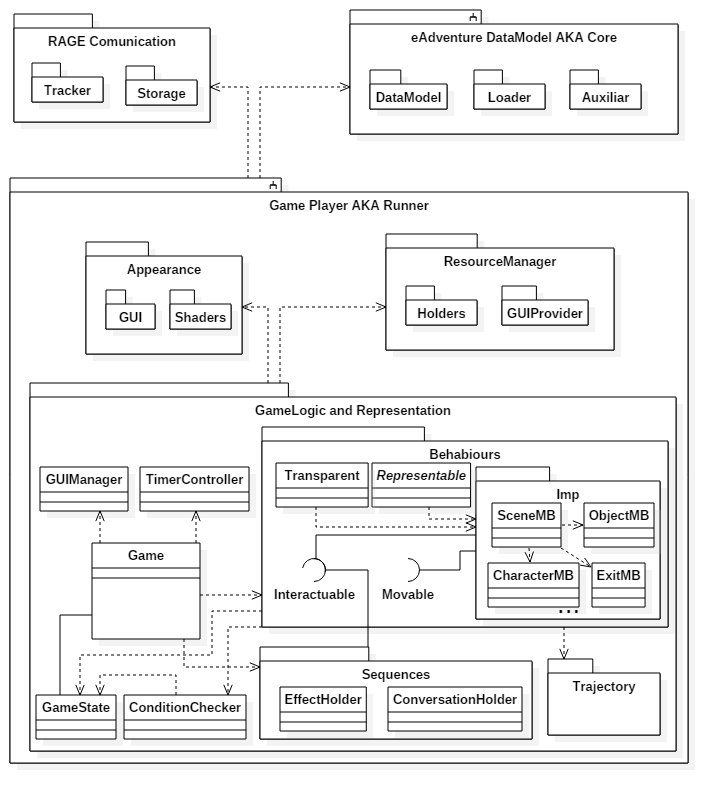
\includegraphics[height=7.5in]{figures/it2/Arquitectura.png}}
	\caption[Arquitectura - Versión Final]{Arquitectura del sistema, a nivel de paquetes de la versión final del proyecto}
	\label{arquitecturait2}
\end{figure}

\newpage

\section{El núcleo de Ejecución: Runner}
\label{runnerit2}

El núcleo de ejecución, también conocido como \textit{Runner}, está dividido en 3 subpaquetes, \textit{Apearance}, encargado de mejorar la representación visual, \textit{ResourceManager}, encargado de realizar la carga transparente de recursos, y \textit{GameLogic}, el cual podría considerarse el núcleo en si mismo, de lógica del juego. Estos tres paquetes surgen de la generalización de elementos que se encontraban, o bien en la antigua clase \textit{Game}, explicada en la sección \ref{gameit1}, o bien en alguna de las clases de utilidad, explicadas en la sección \ref{utilit1}.

De esta manera conseguimos que, la antigua clase controladora del juego \textit{Game}, y las Clases de Utilidad, ahora no tenga que realizar tantas tareas como realizaba anteriormente. En su lugar surgen 5 clases. Estas clases se encargan de hacer transparente la gestión de diversas tareas. Algunas de ellas realizan la gestión de un elemento en concreto, otras controlan la ejecución de otros elementos, y, por último otras se encargan de gestionar el estado del juego.

Estas 5 clases son:
\begin{enumerate}
	\item \textbf{Game}: La clase Game ha sido reducida para encargarse de tres tareas principales: En primer lugar, iniciar la carga y poner en funcionamiento el juego una vez esté cargado. En segundo lugar, controlar la interacción del usuario con los elementos del juego, ya sean elementos con representación, o elementos abstractos como secuencias. Y por último, ser la puerta de enlace que permite elegir qué escena se va a representar.
	
	\item \textbf{GUIManager}: Este gestor se encarga de realizar la gestión de la interfaz que antes se realizaba en \textit{Game}. Permite la emisión de burbujas de diálogo y el control sobre ellas, la posibilidad de mostrar una lista de opciones entre las que el usuario debe seleccionar una respuesta, y por último, la representación de acciones, como botones, y la gestión del menú contextual.
	
	\item \textbf{GameState}: Aunque \textit{GameState} no se considere un \textit{Manager} en si mismo, porque, a diferencia de todos los demás, no es un Singleton, siempre sigue habiendo una única Instancia, pues solo podemos tener un estado de juego, excepto cuando cargamos y guardamos partida. Maneja el estado del juego, que antes se realizaba en \textit{Game}, y facilita funciones para acceder a objetos de la especificación del juego, como \textit{Item} o \textit{NPC}.
	
	\item \textbf{TimerController}: Este gestor que se encarga de controlar los temporizadores que se utilizan en uAdventure para determinadas tareas, como, por ejemplo, hacer que un edificio se queme si no se ha evacuado a tiempo, es, tanto un \textit{Singleton}, como un \textit{MonoBehaviour}, pues necesita de la función \textit{Update()} para controlar que sus temporizadores no hayan saltado. Esta funcionalidad no estaba disponible en la anterior iteración.
	
	\item \textbf{ResourceManager}: este gestor se encarga de facilitar un repositorio transparente a través del cual acceder a los recursos del juego. Añade funcionalidades adicionales que no estaban disponibles anteriormente, como la persistencia en memoria de recursos para agilizar los tiempos de carga, la carga de vídeos, así como la carga de archivos de sonido.
\end{enumerate}

La representación de las clases que se explican en esta sección está disponible en la figura \ref{runnerbigit2}, junto a todas sus funciones. En este diagrama no están representados todos los elementos, pero si aquellos que han surgido de la evolución de las clases que se especificaron al comienzo de la sección. Este diagrama es bastante específico, pues contiene datos acerca de todas las funciones disponibles en cada uno de los elementos.

\newpage

\begin{figure}[h!]
	\centerline{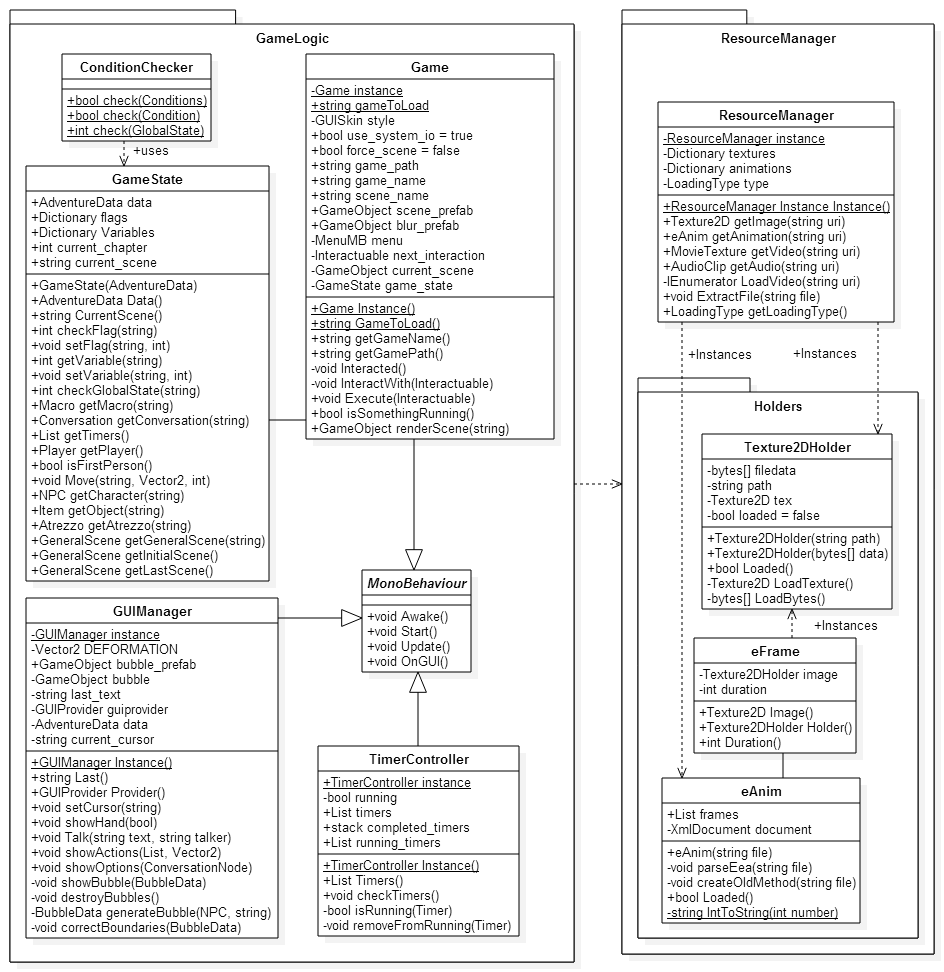
\includegraphics[height=7.5in]{figures/it2/GameLogicBigOnes.png}}
	\caption[GameLogic Grandes Gestores - Versión Final]{Diagrama de clases de los grandes gestores que controlan y proveen contenido para la ejecución del juego.}
	\label{runnerbigit2}
\end{figure}

\newpage

\subsection{El estado del juego: GameState}

Antes de explicar la clase \textit{Game}, es importante explicar la clase que realiza de nexo de unión entre eAdventure y uAdventure, pues esta tiene dos tareas principales: controlar el estado del juego, sus variables, las \textit{Flags} que definen hitos; y la tarea de facilitar el acceso a elementos del juego como los personajes que hay en el capítulo que está siendo jugado en ese momento, como la escena inicial o final de dicho capítulo.

En esencia \textit{GameState} provee un acceso transparente a la especificación del juego en ese momento. Si le pides un personaje, te va a dar la representación de ese personaje en el capítulo que estés jugando. Es importante la relación de asociación direccional que se ve en la figura \ref{gamestateit2} entre \textit{Game} y \textit{GameState}, pues la clase controladora del juego necesita un estado del juego para funcionar, y sin ella, el juego no puede ejecutarse.

\begin{figure}[h!]
	\centerline{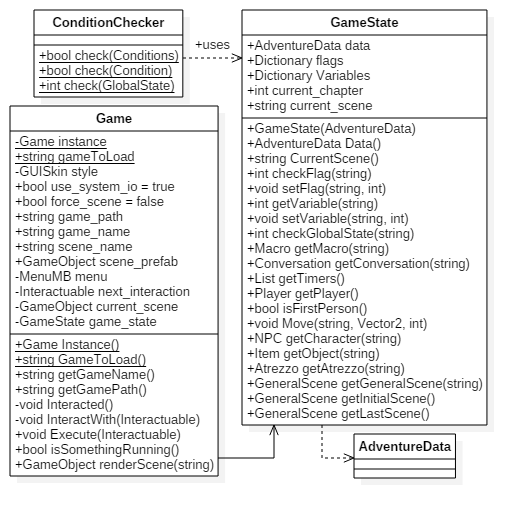
\includegraphics[height=4in]{figures/it2/GameState.png}}
	\caption[GameState - Versión Final]{Diagrama de clases de GameState, junto a Game, ConditionChecker y AdventureData}
	\label{gamestateit2}
\end{figure}

\subsubsection{El validador de Condiciones: ConditionChecker}

Adicionalmente, se muestra en la figura \ref{gamestateit2} a una pequeña clase estática llamada \textit{ConditionChecker}, que se encarga de facilitar la validación de condiciones y estados globales de eAdventure, estas condiciones pueden estar compuestas por multitud de comprobaciones de \textit{Flags} o Variables dentro del \textit{GameState}, por lo que este validador facilita y simplifica mucho el acceso a \textit{GameState}.

\subsection{El Controlador del Juego: Game}
\label{gamesectionit2}

La clase \textit{Game}, ha evolucionado de la clase explicada en la sección \ref{gameit1}. Como se ha mencionado multitud de veces a lo largo de la sección \ref{arquitecturait2}, esta clase \textit{Game} ha evolucionado para delegar comportamientos en los 5 grandes gestores. Sin embargo, la funcionalidad que \textit{Game} aporta en el ciclo de vida y ejecución del juego sigue siendo de vital importancia.

Esta clase \textit{Game} ahora se encarga de 3 tareas: iniciar la carga y poner en funcionamiento el juego una vez esté cargado; controlar la interacción del usuario con los elementos del juego, así como con efectos y conversaciones; y ser la puerta de enlace que permite elegir qué escena se va a representar. No obstante estas tres tareas son vitales, pues en esencia, un juego sólo se puede jugar si se trata esta funcionalidad.

Como la clase \textit{Game} es la puerta de enlace que transforma de una clase \textit{AventureData} a algo jugable, junto a la explicación de \textit{Game}, como subapartados, se presentarán los comportamientos encargados de enrolarse como los diferentes elementos que forman las escenas de eAdventure.

Uno de los cambios más notorios en todo el núcleo de representación es la desaparición de las Clases de Datos explicadas en la sección \ref{dataclassesit1}. Esto es debido a la incorporación del modelo de datos original portado directamente de eAdventure.

En la figura \ref{gameit2} se muestra un diagrama de clases que explica las relaciones de las clases que participan en esta representación del juego. Aunque \textit{SceneMB} tenga una relación de dependencia con \textit{Game}, la escena únicamente necesita acceder a \textit{GameState}, para obtener las especificaciones de los elementos que va a instanciar. \textit{SceneMB} a su vez mantiene relación de dependencia con \textit{PlayerMB}, \textit{CharacterMB}, \textit{ObjectMB}, etc... debido a que \textit{SceneMB} instancia todas estas clases como hijas suyas.


\begin{figure}[h!]
	\centerline{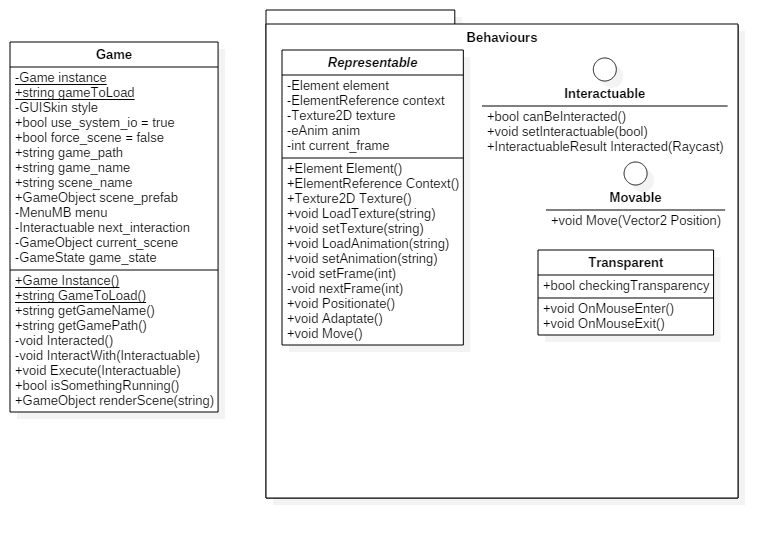
\includegraphics[height=7.2in]{figures/it2/Game.png}}
	\caption[Game - Versión Final]{Diagrama de clases de Game, con todo el nucleo de representación}
	\label{gameit2}
\end{figure}

\subsubsection{Representable, Interactuable, Movable y Transparent}

Este grupo está compuesto por dos clases y dos interfaces, y permiten a la implementación de los comportamientos facilitar la definición de lo que pueden y no pueden hacer. Las dos interfaces son Interactuable y Movable. Tras esto encontramos Representable como clase abstracta que ayuda a la representación de todos los elementos que utilizan recursos, facilita la relación con el \textit{ResourceManager}, y, al extender la clase \textit{MonoBehaviour}, permite a todos los elementos que la extienden ser componentes a su vez. Por ultimo tenemos la clase \textit{Transparent} que, facilita la interacción con elementos que, por motivos de representación en su imagen, no ocupan toda la imagen, teniendo transparencia.

En primer lugar, hablando de \textit{Interactuable}, es la interfaz que permite a \textit{Game} la interacción entre el usuario y los elementos de la escena. \textit{Game}, cuando detecta una pulsación de ratón, lanza un rayo desde dicha posición, en dirección en la que mira la cámara, obtiene una lista de objetos, y, si implementan la interfaz \textit{Interactuable}, les notifica que se ha realizado una interacción con ellos. Estos tienen tres opciones que responder: que no van a hacer nada con la interacción, que hacen algo con ella, o que hacen algo y además esperan más por parte del usuario. En el momento en que \textit{Game} detecta alguna que hace algo, deja de notificar a los demás.

En segundo lugar, hablando de \textit{Movable} es una interfaz sencilla que deben implementar todos aquellos elementos que deseen moverse. Y que únicamente tiene un método \textit{Move()}

En tercer lugar, hablando de \textit{Representable}, encontramos la clase abstracta más compleja, pues permite a los elementos anteriormente citados representarse. Por si misma no realiza ninguna tarea, necesita que la clase que la extienda le indique lo que necesita. Por ejemplo, un objeto de Atrezzo, en su función \textit{Start()} realiza lo siguiente:

\begin{lstlisting}
void Start()
{
	base.Start ();
	base.setTexture(Atrezzo.RESOURCE_TYPE_IMAGE);
	base.Positionate ();
}
\end{lstlisting}

Además de esto, \textit{Representable}, se encarga de transformar esa línea de especificación de recurso \textit{Atrezzo.RESOURCE\_TYPE\_IMAGE} en una \textit{Texture2D} mediante el uso del \textit{ResourceManager}. Asimismo, esta clase \textit{Representable} tiene también facilidades para el uso de animaciones y su actualización en fotogramas.

Finalmente, hablando de la clase \textit{Transparent} es una componente que se añade a los objetos de la escena, y tiene una relación de dependencia con ellos, ya que, sin esta clase, nunca se habilitarían dichos objetos para permitir la interacción con ellos. En \textit{Transparent} se analizan los píxeles de la textura activa en \textit{Representable}, y, si el píxel sobre el cual se tiene el ratón no es transparente, es decir, su componente \textit{Alpha} de color es mayor que 0, se accede a \textit{Interactuable} y se establece como que se puede realizar interacción con dicho elemento.

Estos cuatro elementos de los que se componen los objetos de la escena están representados en la figura \ref{behavioursit2}, con sus relaciones.

\begin{figure}[h!]
	\centerline{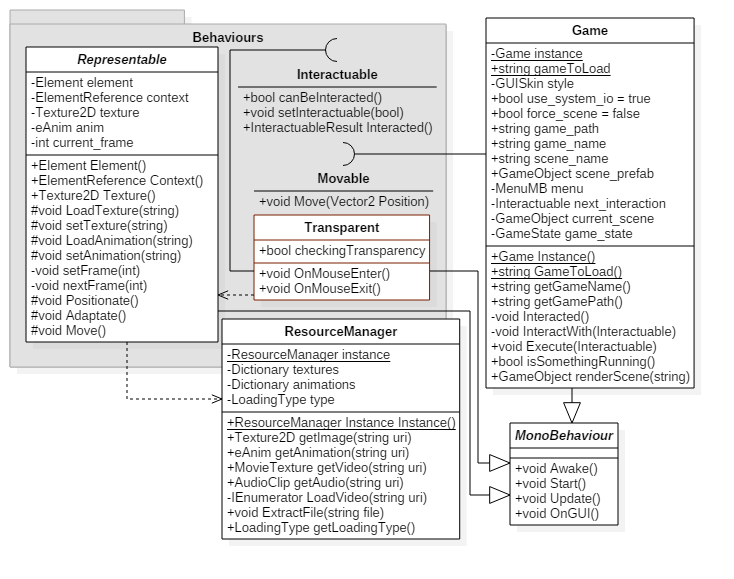
\includegraphics[height=4in]{figures/it2/Behaviours.png}}
	\caption[Representable, Interactuable, Movable y Transparent - Versión Final]{Diagrama de clases de Representable, Interactuable, Movable y Transparent}
	\label{behavioursit2}
\end{figure}

\newpage

\subsection{La escena y sus elementos}

La escena de eAdventure, además de poder ser de multitud de tipos diferentes, está llena de elementos, algunos de ellos que están "vivos", otros que permiten interacción, y otros que únicamente son elementos que mejoran la representación visual. En conjunto, todos estos elementos permiten representar lo que se desee dentro de un escenario. Los elementos que se presentan en esta sección evolucionan de los explicados en la sección \ref{behavioursit1}.

En esta sección se remarcan las diferencias entre las clases de comportamiento presentadas en la sección \ref{behavioursit1} y las actuales, especificando cómo han evolucionado estas. En esencia, su funcionalidad se ha mantenido, o delegado en otras clases, así como han ganado funcionalidad extraída de la clase \textit{Game}. Esto es debido a que siguen siendo los mismos elementos que conforman la escena.

Otro detalle es, para diferenciar más fácilmente entre las clases del modelo de datos y los comportamientos, se les han añadido las siglas MB de \textit{MonoBehaviour}, que identifican que son comportamientos y no clases de datos.

\subsubsection{Detalles de la escena: SceneMB}
\label{scene}

La escena ha sido refactorizada y ampliada para incluir más funcionalidad y facilitar el uso de otra. Detalles de esto se puede encontrar en la figura \ref{gameit2}.

En primer lugar, ahora la escena da soporte a vídeos, aunque estos vídeos han de estar en formato OGV\footnote{El formato OGV es el contenedor de archivo de vídeo que utiliza el códec libre de video Theora.}. Se ha realizado una investigación para determinar si es posible realizar una conversión del formato de los vídeos y su explicación se encuentra en la sección dedicada a la tercera iteración del proyecto.

En segundo lugar, la escena ha simplificado la instanciación de sus elementos, e implementa dos métodos para dicha tarea, los cuales son:

\begin{lstlisting}
private void instanceElement<T>(ElementReference context) where T : Element
private void instanceRectangle<T>(Rectangle context) where T : Rectangle
\end{lstlisting}

Estas funciones, pese a ser funciones tipadas, tienen la peculiaridad de delimitar el tipo de clases que admiten. Esto se consigue utilizando \textit{where T : Interface}.

En tercer lugar, como ahora el juego tiene soporte a juegos en tercera persona, en los que el jugador forma parte de la escena, esta ahora puede contener trayectorias para que el jugador se pueda mover sobre ellas. El cálculo de estas trayectorias fue una de las tareas más complejas de implementar, y se explica en la sección \ref{trajectoryit2}.

Por último, ahora la escena gestiona la interacción que se realice sobre ella, aunque es diferente dependiendo de qué tipo de escena se esté mostrando:
\begin{itemize}
	\item \textbf{Scene}: Si la escena es una escena normal, y además el juego es en tercera persona, se busca el punto que sea más cercano a la trayectoria, se calcula una ruta para que el jugador llegue a ese punto, y se le indica al jugador que inicie el movimiento dada dicha ruta.
	
	\item \textbf{SlideScene}: Si la escena contiene diapositivas, pasaremos a la siguiente diapositiva. Si por el contrario ya no quedan, se continuará a la escena que la siga, ya sea la anterior o una nueva.
	
	\item \textbf{VideoScene}: Si se recibe una interacción, se para el vídeo, y se continúa cargando la siguiente escena igual que en una \textit{SlideScene}.
\end{itemize}

\subsubsection{Los objetos del juego: ObjectMB}
\label{itemsit2}

Con respecto a lo explicado en la sección \ref{objectexitactiveareait1} acerca de la antigua clase \textit{eObject}, esta ha sufrido una evolución. Se ha simplificado mucho gracias al uso de \textit{Representable}, \textit{Interactuable} y \textit{Transparent}. Ahora únicamente reacciona si la componente \textit{Transparent} se lo permite, y gracias a \textit{Representable} y al \textit{ResourceManager} es mucho más sencillo cambiar entre la textura normal y la textura activa, que se debe mostrar cuando el ratón pasa por encima el objeto.

Por otra parte, los objetos implementan una nueva funcionalidad, que les permite ser arrastrados en vez de generar un menú contextual cuando se interactúa con ellos. La especificación de cuándo esto debe suceder se encuentra en la propia especificación del \textit{Item} que se está representando. Se remarca lo descrito en la sección \ref{gamesectionit2} acerca de la desaparición de las clases de datos descritas en la sección \ref{dataclassesit1}, y la sustitución de las mismas por el modelo de datos de eAdventure.

\subsubsection{Las deformables ActiveAreasMB}
\label{activeareasectionit2}

Como se ha mencionado en secciones anteriores, en la versión final, las \textit{ActiveAreas} adquieren la capacidad de deformarse. Esto se consigue gracias a la utilización del Área de Influencia facilitado en la especificación del \textit{ActiveArea}.

En la función \textit{adaptate()}, una \textit{ActiveArea} se encarga de leer esta \textit{InfluenceArea}, y transformar estos puntos, que se encuentran en coordenadas relativas a la escena, a puntos colocados alrededor del centro de ellos. Tras esto se utiliza la libreria \textit{LibTessDotNet} que genera una lista de triángulos a partir de esos puntos.

Una vez se obtienen los puntos y la lista de triángulos, se genera una nueva malla tridimensional estableciendo los vértices en dicha malla, y los triángulos en forma de referencias a los índices de la lista de vértices. Una vez generada dicha malla, se intercambia la \textit{SharedMesh}\footnote{La SharedMesh es una componente de los objetos tridimensionales de Unity3D que contiene la malla tridimensional que lo representa.} por la nueva malla, consiguiendo como resultado un objeto tridimensional con la forma deseada.

Finalmente, este elemento de la escena, como muchos otros elementos interactivos, tienen una componente \textit{AutoGlower}, la cual se explica en la sección \ref{apearanceseccionit2}, que hace que brillen durante un instante cada intervalo regular de tiempo.

Esto se ve representado en la figura \ref{activeareasit2}. Las figuras blancas son las áreas de influencia que dan forma a dichas areas activas. Estas capturas han sido obtenidas del juego utilizado para formar acerca de los primeros auxilios, desarrollado por Catedu.

\begin{figure}[h!]
	\centerline{\includegraphics[height=3in]{figures/it2/Apearance/ActiveAreas.png}}
	\caption[ActiveAreas - Versión Final]{Representación de las ActiveAreas en el videojuego FirstAid}
	\label{activeareasit2}
\end{figure}

\subsubsection{Las clases vivas: PlayerMB y CharacterMB}
\label{playerit2}

De las clases mostradas anteriormente, existen dos clases que implementan la interfaz \textit{Movable}, pues necesitan moverse por la escena. Estas son \textit{CharacterMB} y \textit{PlayerMB}.

En esencia estos dos elementos de la escena son iguales, salvo por la peculiaridad de que \textit{CharacterMB} permite interactúar con el, y realizar acciones que requieran la interacción con ella. Como dicha interacción es trivial, únicamente se explica la parte relacionada con la gestión del movimiento y animaciones.

En primer lugar, cuando en una de estas clases es invocada la función \textit{Move()}, se genera una cola de puntos a los que se debe ir. Tras esto se establece el primer nodo de la cola como nodo destino, y, dependiendo de la dirección hacia la que se deba desplazar para alcanzar dicho nodo, se muestra una animación u otra. Cuando el movimiento se completa y se alcanza el nodo destino, el siguiente nodo de la cola pasa a ser el nodo objetivo, y se realiza el mismo proceso hasta completar la cola de nodos. 

En segundo lugar, cuando una de estas es llamada a hablar, si esta tiene animaciones para el diálogo, se activan mientras la burbuja de diálogo siga activa.

\subsubsection{Las trayectorias: TrayectoryHandler}
\label{trajectoryit2}

La gestión de las trayectorias dentro de la escena es una de las labores más complejas de realizar, pues, en general, los algoritmos de búsqueda de rutas suelen ser algoritmos complejos, y la interacción con una trayectoria, que es algo simbólico, una lista de puntos en el espacio, unidos por líneas, es una tarea compleja.

Por ello, para la gestión de trayectorias, se han implementado 3 clases necesarias para funcionalidades concretas:

\begin{enumerate}
	\item \textbf{TrajectoryHandler}: esta clase es la encargada de proveer el manejo de una \textit{Trajectory} de eAdventure. Se genera a partir de una de estas, y facilita funciones capaces de generar rutas entre puntos que se encuentren en dichas trayectorias.
	
	\item \textbf{LineHandler}: esta clase se encarga de la gestión de una Línea de trayectoria. Está compuesta por dos nodos y la línea que los une. Tiene funciones para determinar que líneas son vecinas de esta línea, cuales son los puntos de contacto a partir de otro punto, o si saber si un punto está contenido en dicha línea.
	
	\item \textbf{MathFunction}: esta clase, dados dos puntos de una recta, mediante el uso de funciones matemáticas, es capaz de generar un valor Y para una X dada, o un valor X para una Y dada, así como es capaz de generar puntos de contacto a partir de otro punto.
\end{enumerate}

El tratamiento de trayectorias comienza con la generación de un \textit{TrajectoryHandler}, este analiza dicha trayectoria, y para cada lado de esta genera un \textit{LineHandler}. Una vez que todos han sido generado, se llama a la función \textit{UpdateNeighbors()} que recorre esta lista de líneas y, si dos líneas contienen extremos comunes, se determina que estas son vecinas.

Las líneas, cuando son generadas, utilizan sus dos puntos para generar una \textit{MathFunction} que les ayudará a generar y a determinar puntos que estén en su línea.

Lo complejo del tratamiento de trayectorias llega con el cálculo de rutas. Para ello se ha implementado una variante del algoritmo de Dijkstra para hallar caminos mínimos en grafos no direccionales con coste. La diferencia es que, debido a que en la ruta el nodo inicial y el nodo final no forman parte de la trayectoria en si misma, sino que son nodos nuevos que se generan en tiempo de ejecución, y únicamente se identifica en qué líneas de trayectoria están contenidos dichos puntos.

Tras esto se identifica que líneas contienen el punto de origen y el punto destino, y con esto se realiza el algoritmo de marcado de Dijkstra pero únicamente utilizando las líneas, sin los nodos. Y finalmente se ejecuta la función \textit{reach()} que prepara el lanzamiento de la función recursiva de mismo nombre encargada de recorrer el grafo siguiendo la especificación del algoritmo de Djikstra.

No obstante, el funcionamiento de este algoritmo no es tan bueno como se desearía, pues le falta incluir la distancia que hay entre el punto de origen o destino, y el nodo inicial elegido de la línea de origen y destino. Asimismo, se pueden dar resultados no optimos. Como trabajo futuro se plantea implementar el algoritmo de Djikstra con nodos, e incluir los nodos origen y destino en la trayectoria.

\begin{figure}[h!]
	\centerline{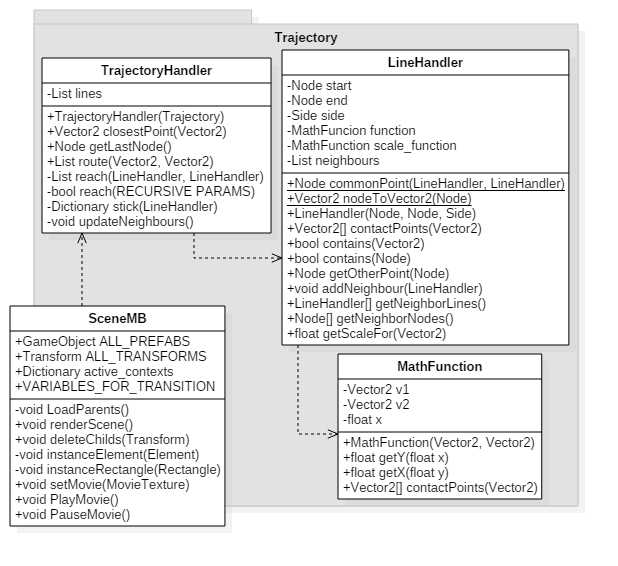
\includegraphics[height=3.7in]{figures/it2/TrajectoryHandler.png}}
	\caption[TrajectoryHandler - Versión Final]{Diagrama de clases de las trayectorias, junto a LineHandler y MathFunction}
	\label{trajectoryfigit2}
\end{figure}

\subsection{Las secuencias: Effect y GraphConversation}
\label{sequencesit2}

La implementación de las secuencias, visible en la figura \ref{sequencesfigit2}, tanto de efectos, como de conversación cambió mucho desde la primera iteración hasta la segunda iteración. En esencia, se han eliminado las factorías de efectos, pues estas ya no necesitan ser autogeneradas a partir del fichero de especificación en XML, pues el paquete \textit{Loader} del modelo de eAdventure ya se encarga de realizar dicha lectura.

Sin embargo, siguen manteniendo la esencia, y no se ha implementado ningún \textit{SequenceManager} que se encargue de ejecutar las secuencias. En su lugar, siguen siendo autoejecutables, siendo más sencillo de recordar estados si la escena se para en la mitad de su ejecución y a su vez contiene llamadas a secuencias dentro de si mismas.

Mas allá de esto, el esfuerzo se realizó añadiendo la mayor parte de efectos disponibles en eAdventure, y únicamente dejando unos pocos por implementar, y por otra parte, haciendo funcionar los \textit{Holders}, con las clases del modelo de datos de eAdventure.

\begin{figure}[h!]
	\centerline{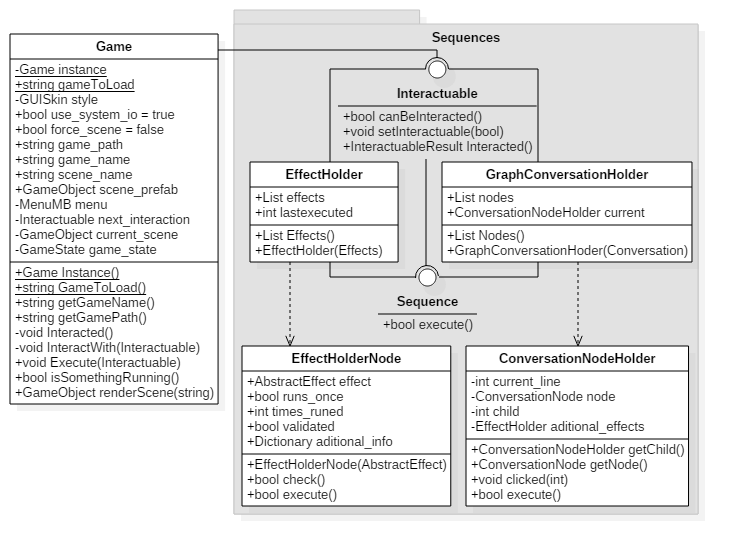
\includegraphics[height=3.7in]{figures/it2/Sequences.png}}
	\caption[Sequences - Versión Final]{Diagrama de clases de las Secuencias, mostrando tanto EffectHolder como GraphConversationHolder}
	\label{sequencesfigit2}
\end{figure}

\subsection{El controlador de los temporizadores: TimerController}
\label{timercontrollersecit2}

El controlador de los temporizadores es una clase nueva que no existía en la anterior iteración. Esta clase comportamiento se añade como componente a la cámara y se encarga, mientras está contando, de controlar los \textit{Timers} que el juego necesita para su ejecución.

Para manejar los temporizadores se ha implementado un enumerado llamado \textit{TimerType} que establece el tipo de temporizador que se está tratando, y una clase llamada \textit{TimerState} que únicamente sirve para almacenar datos acerca de los temporizadores que se encuentran en ejecución.

Este controlador tiene además la opción de parar su ejecución para que, si el juego se encuentra parado esperando a que el jugador interactúe en una secuencia, no salten temporizadores en mitad de dicha secuencia. 

Para gestionar estos temporizadores se tienen tres listas:  una lista con todos los temporizadores de dicho capítulo, una lista con los temporizadores que están ejecutándose, y por último una cola con los que ya se han completado.

Se aprovecha de la función \textit{Update()} de \textit{MonoBehaviour} para controlar el paso del tiempo en los mismos, así como detectar qué temporizadores cumplen las condiciones para ejecutarse, y cuáles de los que se encuentran en ejecución ya no deberían estar ejecutándose.

\begin{figure}[h!]
	\centerline{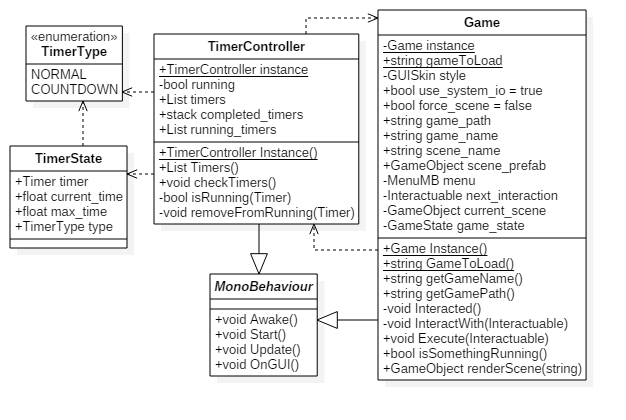
\includegraphics[height=4in]{figures/it2/TimerController.png}}
	\caption[TimerController - Versión Final]{Diagrama de clases de TimerController, incluyendo las clases y enumerados para su funcionamiento.}
	\label{timercontrollerit2}
\end{figure}

la figura \ref{timercontrollerit2} muestra el diagrama de clases de lo descrito anteriormente. En este diagrama se ve como \textit{Game} establece los \textit{Timers} que deben ser controlados al inicio de cada capítulo, y \textit{TimerController} únicamente los gestiona. Cuando alguno de estos \textit{Timers} se completa, \textit{TimerController} le dice a \textit{Game} que ejecute los efectos de dicho temporizador.

\newpage

\subsection{El gestor de interfaz: GUIManager}
\label{guimanagersectionit2}

Como se explica en la sección superior a esta subsección, existe una clase gestora que se encarga de manejar la interfaz en su totalidad de forma transparente. Facilita una serie de funciones que permiten, de forma sencilla, mostrar burbujas de diálogo, cambiar el cursor, mostrar un menú contextual de acciones, o un menú de opciones.

Este gestor surge de la reducción de contenido de \textit{Game}, que antes realizaba estas tareas, y fue relevada de su función debido a que dicha clase comenzaba a tener una dimensión demasiado elevada. La figura \ref{guimanagerit2} muestra el diagrama de clases de la clase \textit{GUIManager} junto al paquete \textit{Apearance}, el paquete \textit{GUIProvider} que contiene todo lo necesario para acceder al \textit{ResourceManager} de forma automática y transparente, así como la carga de recursos por defecto y la gestión de nombres a constantes y viceversa, y el paquete \textit{Menu}, que contiene una serie de clases para la representación y animación del Menú.

Este gestor hereda de \textit{MonoBehaviour}, por lo que es asignado como componente de un elemento dentro de la escena. En este caso se asigna a un objeto \textit{Canvas}, que permite la representación de elementos de interfaz. 

El ciclo de vida de \textit{GUIManager} comienza cuando despierta la escena. En este momento se establece como instancia a si mismo. Tras esto, cuando \textit{Game} ya ha cargado el juego, y se ejecuta la función \textit{Start()}, este provee al \textit{GUIProvider} de los datos del juego en forma de un \textit{AdventureData}. Este se prepara y carga los recursos que deba cargar, y tras esto, el \textit{GUIManager} se queda en espera hasta que el juego necesite mostrar al usuario algo.

Una vez que el \textit{GUIManager} se encuentra en espera, facilita una serie de funciones útiles para representar cosas al usuario, estas son:
\begin{itemize}
	\item \textbf{Talk(string line, string talker)}: Esta función permite al sistema que los personajes hablen. Esto se ha implementado mediante el uso de burbujas.
	
	\item \textbf{showActions(List<Actions>, Vector2 position)}: Esta función pone en ejecución al menú contextual, y hace que se muestre con las acciones especificadas en una posición.
	
	\item \textbf{showOptions(ConversationNode)}: Esta función permite mostrar un listado de opciones de texto que el usuario debe elegir. Adicionalmente, el fondo se emborrona y se muestra el texto de la última pregunta.
	
\end{itemize}


\begin{figure}[h!]
	\centerline{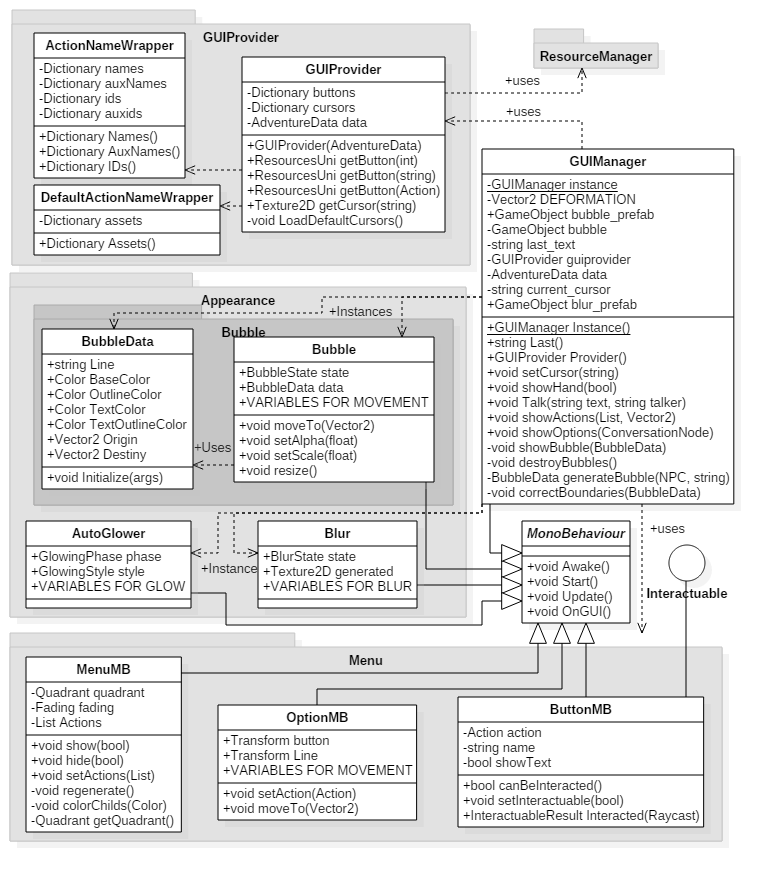
\includegraphics[height=7.5in]{figures/it2/GUIManager.png}}
	\caption[GameLogic Grandes Gestores - Versión Final]{Diagrama de clases de los grandes gestores que controlan y proveen contenido para la ejecución del juego.}
	\label{guimanagerit2}
\end{figure}

\newpage

\subsubsection{Proveedor de recursos de GUI: GUIProvider}

La interfaz es una capa de la vista que necesita representación, y por ello, necesita acceder a recursos para poder representarse. Sin embargo, nuestro gestor de \textit{GUI} no usa directamente al \textit{ResourceManager}, sino que utiliza una clase intermedia para acceder a los recursos, esta clase es \textit{GUIProvider}, y se encarga de, facilitar el acceso a texturas que tengan una funcionalidad concreta. Es decir, por ejemplo, obtener la textura que representa a una acción, o el cursor que se debe mostrar para un determinado elemento. \textit{GUIProvider} se encarga de proveer los recursos apropiados.

Además de esto, eAdventure sigue una jerarquía a la hora de definir recursos para la interfaz, esta es la siguiente:

\begin{enumerate}
	\item Se cargan los recursos por defecto. Estos recursos están repartidos en dos directorios, el primero es la carpeta "~/gui/hud/contextual/" donde se encuentran los botones que representan los distintos tipos de acciones y que se obtienen utilizando la clase \textit{DefaultActionNameWrapper}. El segundo el la carpeta "~/gui/cursors/" donde se encuentran los cursores del juego, y que se obtienen utilizando la clase \textit{ActionNameWrapper}. Estas dos clases \textit{Wrapper} se encargan de transformar de Acción, o identificador de Acción a nombre, y viceversa.
	
	\item Se cargan los recursos especificados en la base del archivo "descriptor.xml". Tras la lectura de dicho archivo en \textit{Loader}, estos se encuentran en el objeto de datos \textit{AdventureData} que gestiona \textit{GameState}. Estos también se asignan utilizando los \textit{Wrappers} anteriormente especificados, y, sustituyen a los botones y cursores cargados en el apartado anterior con los que se hayan en esta especificación.
	
	\item Por último puede ocurrir una situación anómala, y es que un elemento tenga una acción personalizada en su interior. En este caso, y excepcionalmente, es el propio botón del menú el que se encarga de solicitar al \textit{ResourceManager} dichos recursos.
	
\end{enumerate}

\begin{figure}[h!]
	\centerline{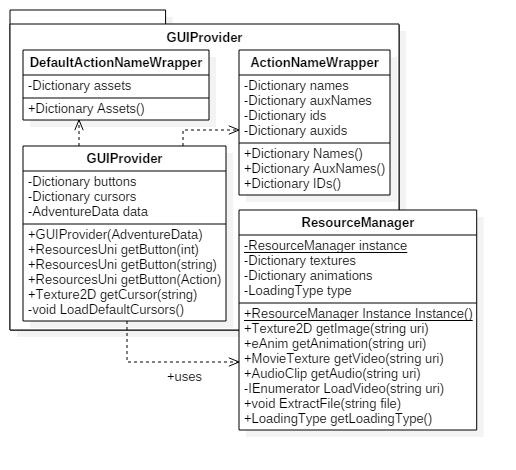
\includegraphics[height=3.5in]{figures/it2/GUIProvider.png}}
	\caption[GUIProvider - Versión Final]{Diagrama de clases de GUIProvider, junto con ResourceManager.}
	\label{guiproviderit2}
\end{figure}

Las clases que participan en este proceso están representadas en la figura \ref{guiproviderit2}. En esta figura, aunque \textit{ResourceManager} esté sobrepuesto al paquete \textit{GUIProvider}, esto es debido a reducir el tamaño del diagrama, realmente este no forma parte de dicho paquete.

\subsubsection{Las burbujas de diálogo: Bubble}

La representación de diálogos en un juego de aventuras es una tarea necesaria, pues los personajes necesitan hablar para compartir información entre ellos. La manera de representar estos diálogos en uAdventure es la misma que se decidió utilizar en eAdventure: Las burbujas de diálogo, o bocadillos de diálogo. Sin embargo, estas burbujas han evolucionado en su representación, realizando una pequeña animación a la hora de ser invocadas, y a la hora de desaparecer.

\begin{figure}[h!]
	\centerline{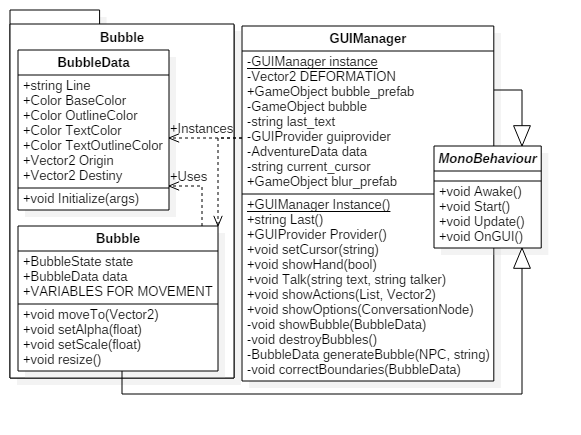
\includegraphics[height=3.5in]{figures/it2/Bubble.png}}
	\caption[Bubble - Versión Final]{Diagrama de clases de Bubble, junto con GUIManager y MonoBehaviour.}
	\label{bubbleit2}
\end{figure}

El proceso de mostrar una burbuja de diálogo comienza en \textit{GUIManager} y es el siguiente: En primer lugar, se identifica si el que habla es el jugador o un personaje, y si es el jugador, se distingue si se trata de un juego en primera persona o un juego en el que el jugador tenga representación en el juego. Una vez se ha determinado quién habla, se obtienen los datos del hablante y se genera una \textit{BubbleData} con dichos datos, decorándola y estableciendo su trayectoria. Este \textit{BubbleData} se pasa a través de una serie de deformaciones que adaptan dichas trayectorias a la pantalla para que no se salga de la misma, y para que se coloque correctamente independientemente de la resolución de la misma. Tras esto se instancia una nueva burbuja en la escena y se delega en ella.

La burbuja, en su función \textit{Start()}, establece su texto en la representación, se prepara para moverse, y se prepara para empezar a mostrarse, pues al principio es transparente. Poco a poco esta se va moviendo y haciéndose visible en su función \textit{FixedUpdate()}, y cuando termina, se queda quieta. Cuando es necesario que la burbuja desaparezca, se ejecuta la función \textit{destroy()} que la hace desaparecer poco a poco, haciéndose más pequeña y transparente.

\subsubsection{Elementos de mejora visual: Apearance}
\label{apearanceseccionit2}

Existen dos clases que, para mejorar la representación visual del juego, se han desarrollado en el proyecto. Cómo se explicó en el apartado \ref{eandroidmokap} del estado del arte, y visible en la figura \ref{eandroidlupa}, el proyecto eAdventure Android utilizaba mecanismos específicos para ayudar al usuario a encontrar elementos en un entorno táctil. En este proyecto, para ayudar al usuario a encontrar estos elementos, se realiza un brillo de los mismos.

La clase componente \textit{AutoGlower} se encarga de realizar este brillo sobre los objetos que la contengan. Tiene varios modos, como simplemente hacer un flash, o aparecerse y desvanecerse y hacer un flash. Este \textit{AutoGlower} utiliza un \textit{Shader} que genera dicho flash y que es parametrizable para establecer tanto la posición del brillo, su color y su anchura. Este efecto es visible en las figuras \ref{autoglow1it2} y \ref{autoglow2it2};

\begin{figure}[h!]
	\centerline{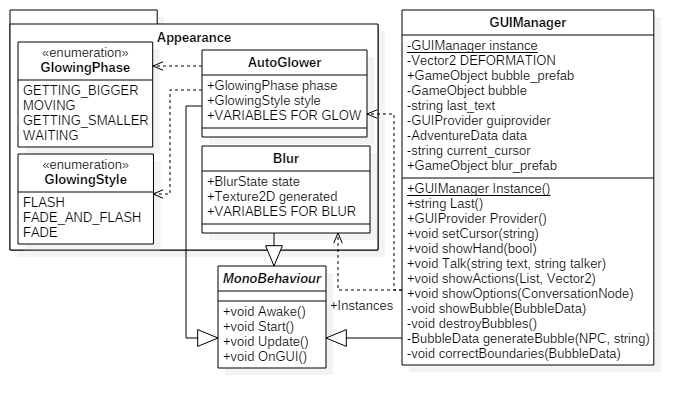
\includegraphics[height=3.5in]{figures/it2/Apearance.png}}
	\caption[Apearance - Versión Final]{Diagrama de clases de Apearance, sin incluir Bubble.}
	\label{apearanceit2}
\end{figure}

Por último, tenemos a la clase \textit{Blur}, que, al igual que la anterior utiliza un \textit{Shader} para conseguir su efecto visual. En este caso, \textit{Blur} lo que hace es volver borroso lo que hay detrás de ella. Es utilizada para generar un cuadrado borroso sobre el cual presentar las distintas opciones disponibles en la lista de opciones de una conversación. Este efecto se puede ver en la figura \ref{blurit2}.

\begin{figure}[h!]
	\centerline{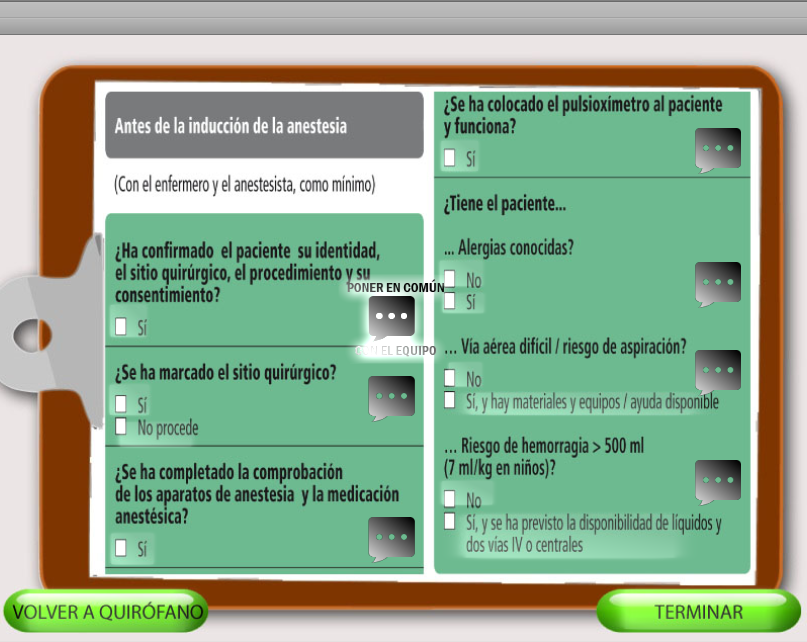
\includegraphics[width=4.3in]{figures/it2/apearance/checklist.png}}
	\caption[Apearance - Versión Final]{Diagrama de clases de Apearance, sin incluir Bubble.}
	\label{autoglow1it2}
\end{figure}

\begin{figure}[h!]
	\centerline{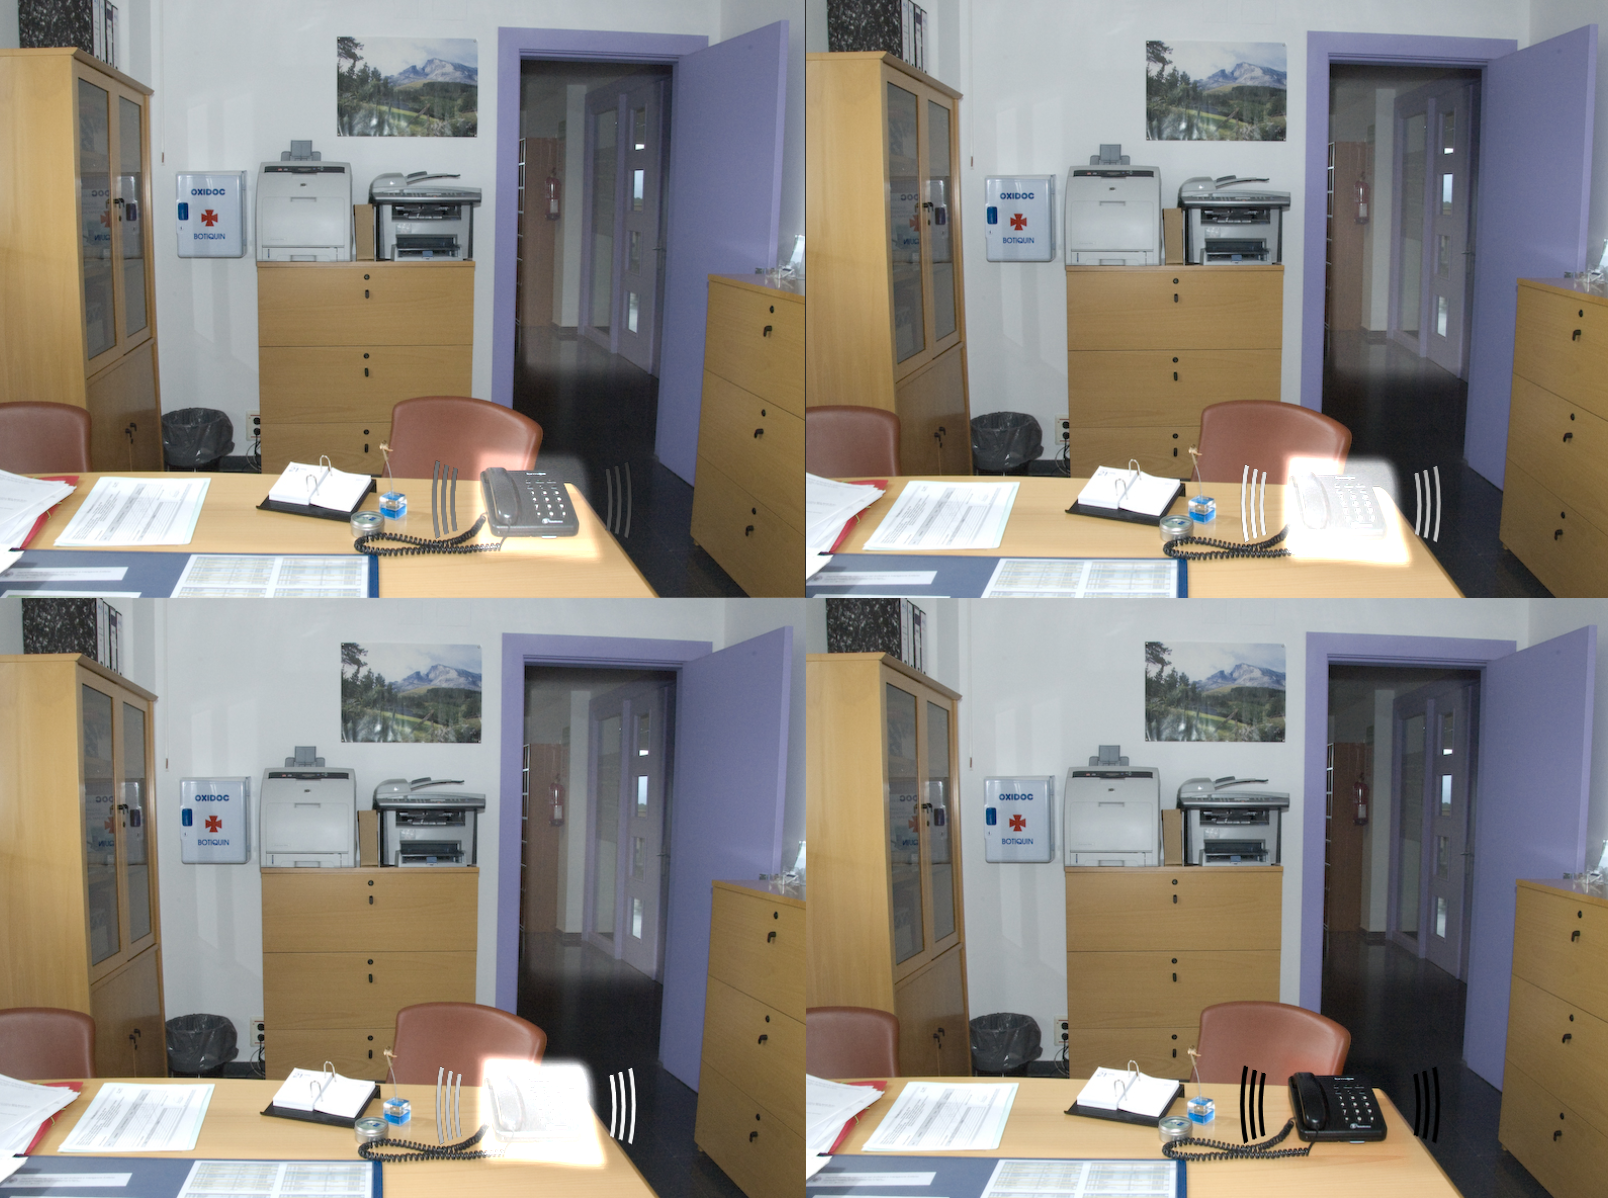
\includegraphics[width=4.3in]{figures/it2/apearance/fire.png}}
	\caption[Apearance - Versión Final]{Diagrama de clases de Apearance, sin incluir Bubble.}
	\label{autoglow2it2}
\end{figure}

\begin{figure}[h!]
	\centerline{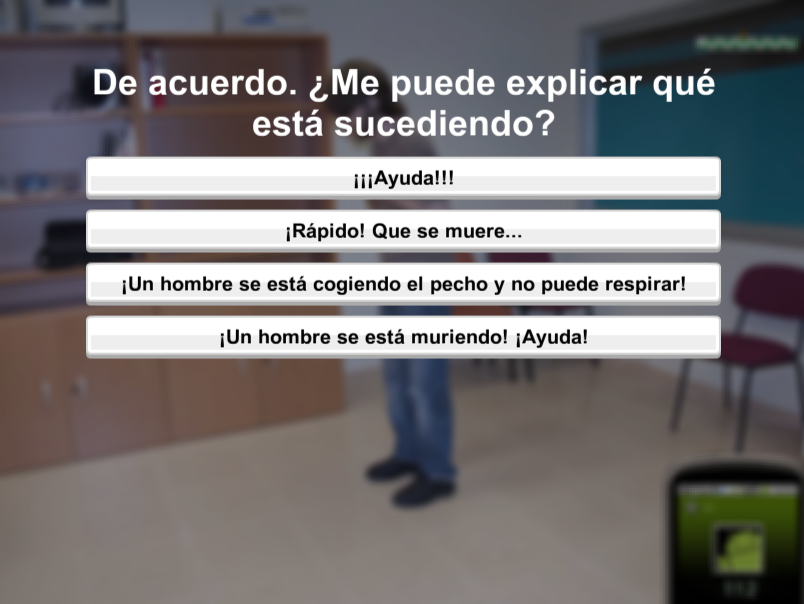
\includegraphics[width=4.3in]{figures/it2/apearance/blur.png}}
	\caption[Apearance - Versión Final]{Diagrama de clases de Apearance, sin incluir Bubble.}
	\label{blurit2}
\end{figure}

\subsubsection{El menú contextual de acciones: Menu}

El menú contextual es uno de los elementos que existían antes y que ha sido recreado, añadiendo animación al mismo para que su representación visual sea más sencilla. La utilidad del menú contextual es mostrar acciones en forma de botones para que el usuario pueda pulsarlos y ejecutar las acciones que están detrás de los mismos.

Este menú contextual se genera utilizando una de las funciones de \textit{GUIManager}, la función \textit{showActions(list<Action>)} que, inicializa el menú y utiliza su función \textit{regenerate()}, que lo que hace es, en función de los parámetros que se le hayan establecido, genera nuevos botones, y los coloca para que se animen correctamente. Tras esto la clase \textit{OptionMB} se encarga de ir colocando tanto la línea que une el centro del menú con el botón, como el botón en si mismo. Asimismo, esta clase establece la acción en \textit{ButtonMB}, clase que implementa la interfaz \textit{Interactuable}, y que permite al usuario interactuar con ella. Es la clase \textit{ButtonMB} la que se encarga de modificar su representación en función de la imagen que le provea el \textit{GUIManager}. Esto está representado en la figura \ref{menuit2}, donde participan \textit{MonoBehaviour} e \textit{Interactuable}.

\begin{figure}[h!]
	\centerline{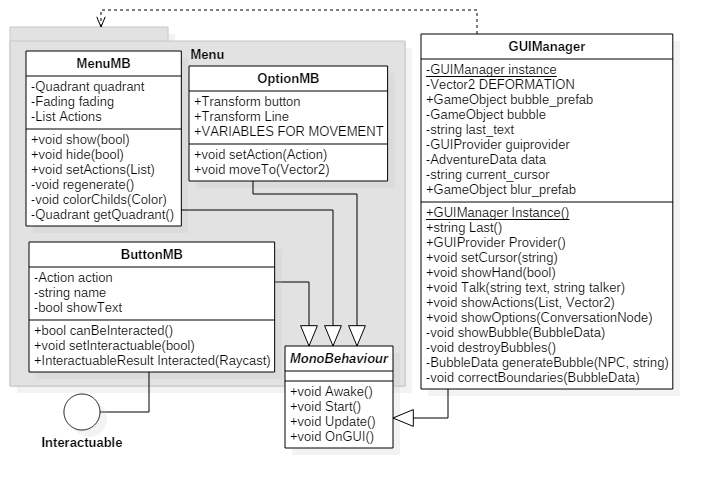
\includegraphics[height=3.3in]{figures/it2/Menu.png}}
	\caption[Menu - Versión Final]{Diagrama de clases de Menu, incluyendo las relaciones que tienen con MonoBehaviour e Interactuable.}
	\label{menuit2}
\end{figure}

Finalmente, en la figura \ref{menuvisualit2} muestra el menú generado en una situación en la que se pueden realizar cinco acciones sobre un elemento de la escena. 

\begin{figure}[h!]
	\centerline{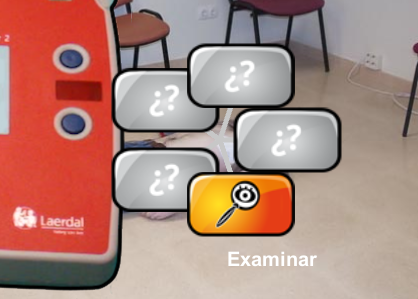
\includegraphics[height=3in]{figures/it2/apearance/menu.png}}
	\caption[Visual Menu - Versión Final]{Imagen de la representación visual del menú.}
	\label{menuvisualit2}
\end{figure}

\subsection{El gestor de recursos: ResourceManager}
\label{resourcemanager}

Como se ha comentado varias veces a lo largo de esta sección, para facilitar el acceso a los recursos desde cualquier parte del proyecto, existe un \textit{Singleton} llamado \textit{ResourceManager} que provee de elementos multimedia al que lo solicite.

Este \textit{ResourceManager} es capaz de cargar múltiples tipos de recursos, y para ello utiliza métodos diferentes. Asimismo, existen dos formas de cargar recursos, y las clases que se encargan de acceder al sistema de archivos para cargar los recursos se adaptan a estos tipos.

Estos tipos de carga, o \textit{LoadingType}, son: utilizando el sistema de ficheros del sistema operativo, mediante la librería \textit{System.IO}, teniendo la ventaja de que, una versión ya generada de uAdventure puede cargar cualquier juego que se establezca en un directorio determinado; y por otra parte, utilizando \textit{Resources.Load()}, mediante el sistema de ficheros de Unity, que tiene la ventaja de que estos archivos, una vez que se produce una \textit{Release} del proyecto, están incluidos en un paquete comprimido por Unity, y permiten instalar uAdventure junto al juego en cualquier plataforma sin tener que preocuparse de incluir el juego.

\begin{figure}[h!]
	\centerline{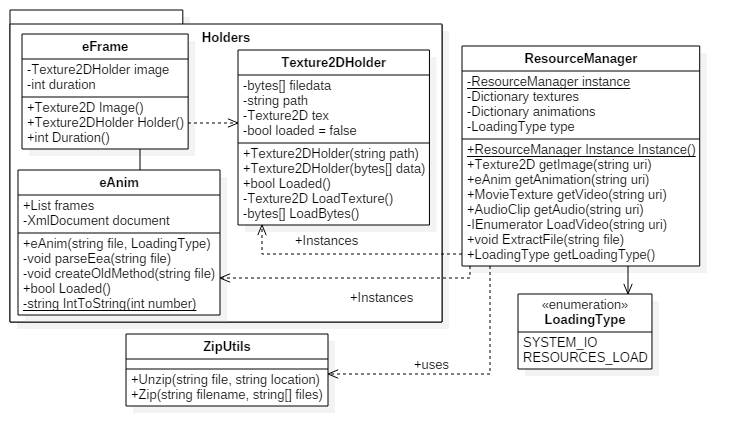
\includegraphics[height=3.5in]{figures/it2/ResourceManager.png}}
	\caption[ResourceManager - Versión Final]{Diagrama de clases de ResourceManager junto a los cargadores de recursos.}
	\label{resourcemanagerit2}
\end{figure}

con respecto a los tipos de ficheros que se pueden cargar con \textit{ResourceManager},encontramos los siguientes tipos:
\begin{itemize}
	\item \textit{Imágenes}: Para la carga de imágenes existe una clase llamada \textit{Texture2DHolder}. Dependiendo del tipo de carga que utilice \textit{ResourceManager}, o bien se carga la textura directamente con \textit{Resources.Load()}, o bien se leen los \textit{bytes} de dicho fichero, para más adelante transformarlos en una \textit{Texture2D}.
	
	\item \textit{Animaciones}: Las animaciones que se cargan son las de eAdventure, y están compuestas por una serie de imágenes, esto se hace en la clase \textit{eAnim}, la cual no ha cambiado mucho en su funcionamiento desde lo explicado en la sección \ref{dataclassesit1}. Para añadir soporte a \textit{Resources.Load()} ha sido necesario implementar un método que renombra todos los archivos ".eaa" a ".xml" pues Unity no reconoce dichos archivos como ficheros de texto y no permite cargarlos.
	
	\item \textit{Vídeos}: La carga de vídeos se realiza almacenándolos en una \textit{MovieTexture}. Para la carga de estos desde el sistema de ficheros se utiliza la clase \textit{www}, que permite hacer solicitudes POST y GET, ya sea en local, al sistema de ficheros, o a un servidor. Esta carga requiere la utilización de corrutinas, pues sin ellas el juego se quedaría completamente congelado hasta que el recurso estuviera cargado. Finalmente mencionar que los vídeos únicamente pueden estar en formato ".ogv" bajo el codec OGG Theora.
	
	\item \textit{Audio}: De manera similar a los vídeos, se utiliza la clase \textit{www} para su carga, aunque en esta ocasión son almacenados en \textit{AudioClip}.
	
	\item \textit{Archivos Zip}: Estos ficheros técnicamente no son cargados en tiempo de ejecución, sino que son extraídos bajo demanda del emulador para importar juegos. Estos juegos deben estar en formato ".jar", y únicamente se extrae de ellos la parte necesaria. Más detalles acerca de este proceso están disponibles en la sección \ref{emulatorit3}.
\end{itemize}

Acerca de los vídeos, y de la importación de los juegos que se realiza en la tercera iteración del proyecto, se realizó una investigación acerca de la posibilidad de transformar dichos vídeos en el proceso de importación del juego. Los resultados no fueron satisfactorios, pero abrieron varias puertas para abordar este problema.

En primer lugar, se probaron multitud de librerías que facilitaban la conversión de vídeos a sistemas .NET, sin embargo, ya que Unity utiliza una versión reducida del mismo, dichas librerías fallaban en tiempo de ejecución y no completaban la conversión del vídeo. Por otra parte, algunas personas que se han enfrentado al mismo problema, han generado \textit{Wrappers} que utilizan un ejecutable del proyecto de software libre \textit{FFMPEG}, que provee de una serie de utilidades para transformar vídeos fácilmente.

Se intentaron incorporar dichos \textit{Wrappers} en el proyecto, pero ninguno de ellos funcionó. Finalmente se decidió que la alternativa de implementar un \textit{Wrapper} muy sencillo, con únicamente la funcionalidad de transformar a OGV, sería la opción mas viable. en windows, esto se haría de la siguiente manera:

\begin{lstlisting}
String path = @"f:\temp\data.txt";
Process foo = new Process();
foo.StartInfo.FileName = "Notepad.exe";
foo.StartInfo.Arguments = path;
foo.Start();
\end{lstlisting}

También existe una manera de lanzar clases Java directamente desde Unity, pudiendo realizar este proceso también en Android, de la siguiente manera:

\begin{lstlisting}
using (AndroidJavaClass ext = new AndroidJavaClass ("com.external.class")) 
{
	ext.CallStatic ("whatever", Parameter1, Parameter2);
}
\end{lstlisting}

Por lo que, como trabajo futuro del proyecto, queda pendiente implementar dicho conversor de vídeos multiplataforma, que utilice diferentes librerías, ya sea \textit{FFMPEG} u otra librería para dicha conversión.

\section{El modelo de Datos: Core}
\label{coreit2}

En el proceso de integración del proyecto de Piotr Marszal que consiste en reconstruir el editor de eAdventure dentro de Unity, se decidió unificar el modelo de datos. En vista de que, para una implementación al completo de todos los elementos del editor, el modelo de datos planteado en la sección \ref{dataclassesit1}, con las clases de datos que eran capaz de generarse a si mismas, era insuficiente para satisfacer las necesidades del proyecto, se decidió invertir mucho tiempo en portar al completo el modelo de datos de las clases Java a Unity.

Esta tediosa y repetitiva labor fue realizada casi en su totalidad por Piotr, quien copiaba el código Java en c\# y se encargaba de sustituir las librerías problemáticas por librerías análogas de .NET. Dentro de mi aportación, se realizaron tareas de corrección de errores y de pruebas para comprobar que todo funcionaba correctamente.

De esta misma manera, Piotr importó el \textit{Loader} original de eAdventure, y, no fue hasta que se comenzó a utilizar en este proyecto, que no se identificó que dicho cargador era inviable de utilizar pues tardaba entre medio y un minuto en leer el documento de especificación del juego; además de que lo hacía con errores que, pese a intentos de arreglarlos, debido a que la implementación de dicho \textit{Loader} fue realizada por uno de los desarrolladores de eAdventure, la complejidad del funcionamiento del mismo se escapaba a nuestra comprensión.

Como estos problemas con el \textit{Loader} continuaban, se decidió crear una nueva implementación del cargador del modelo de datos utilizando la librería \textit{System.XML} que se utilizó para las Clases de datos de la primera iteración, y que ya se conocía que era fácil de utilizar, pues permite utilizar sintaxis de XPath\footnote{XPath (XML Path Language) es un lenguaje declarativo que permite construir expresiones regulares que recorren, procesan y seleccionan elementos de un documento XML}, y acceder al contenido del documento XML de forma sencilla.

Esta segunda implementación la comenzó Piotr, recodificando la mayor parte de \textit{subparsers} del cargador. Sin embargo, el no pudo probar las nuevas clases que estaba implementando, por lo que no pudo darse cuenta de que muchas de ellas, debido a que la base que aplicaba para la transformación no era del todo correcta, no funcionaban. Los grandes \textit{subparsers} como el cargador de escenas, efectos, conversaciones, areas activas, etc... tuvieron que ser nuevamente implementados desde cero por mi. Finalmente, en mi labor se realizó la tarea de implementar los cargadores principales de \textit{AdventureData} y \textit{Chapter}. haciendo estos funcionales al sistema de cargado de ficheros de \textit{System.IO}, así como el de \textit{Resources.Load()}.

Una vez construido el nuevo \textit{Loader}, los tiempos fueron reducidos en un 90\%, pasando de tardar 45 segundos de tiempo de carga en el videojuego \textit{Checklist}, a alrededor de 4 segundos. No obstante esta medida no puede realizarse con precisión debido a que en dichos tiempos de carga se incluye el tiempo que utiliza Unity para inicializarse y ponerse en funcionamiento.

Para completar la integración fue necesario desacoplar partes del sistema de eAdventure entre si mismas, pues el modelo de datos de dicho sistema está extremadamente interconectado, y cada vez que se intenta reutilizar una de sus partes, es necesario traer junto a esa parte, un gran número de partes de dicho modelo. 

Con dicho desacoplamiento, también fueron eliminados del modelo de datos determinados elementos utilizados para iniciar la carga del juego. Por ello fue necesaria una investigación en profundidad hasta hallar una manera segura de trabajar con el paquete \textit{Loader}.

Finalmente, cuando se hubo unificado el modelo de datos, se realizó una unión de ambos proyectos en un único proyecto y repositorio. El proyecto de Piotr se ubica casi en su totalidad dentro del espacio de nombres \textit{Editor}, por lo que, para la unificación de los proyectos, fue necesario extraer de dicho espacio de nombres el modelo de datos, junto al \textit{Loader}, otras clases auxiliares, y más elementos. A esta parte que se extrajo de \textit{Editor} es a la que se conoce como \textit{Core}, pues representa al núcleo de eAdventure.

\newpage

\section{La comunicación con RAGE: RAGETracker}
\label{ragetrackerit2}

Pese a que uno de los objetivos principales de este proyecto es el de garantizar y simplificar el ciclo de vida de los juegos serios producidos con eAdventure, así como extender su vida útil lo máximo posible, otro de los planteamientos con los que surge este proyecto es el de poder mejorar la parte de evaluación de eAdventure mediante el uso de RAGE.

Una de las partes que, por tener un grado de dificultad muy elevado de incluir en Unity, debido a que las librerías que se utilizaban no dan soporte a .NET, y se debe construir una nueva infraestructura para soportarlo, es la parte de \textit{Assessment}. Estas partes, que además no tenían toda la funcionalidad deseada, van a ser sustituidas por \textit{Assessment} con RAGE.

RAGE, Realising an Applied Gaming Eco-system, es un proyecto que apunta a desarrollar, transformar y enriquecer tecnologías específicas para la industria de los videojuegos serios, en forma de paquetes autocontenidos para juegos que ayudan a los estudios de videojuegos en el desarrollo de juegos serios, haciéndolo más sencillo, rápido y eficiente económicamente.

En RAGE hay una parte específica dedicada a la evaluación de videojuegos, y esta parte provee una API para los profesores que deseen crear perfiles de evaluación y progreso, así como otros elementos de utilidad que se deseen monitorizar, como el numero de veces que una pregunta ha sido respondida de forma incorrecta, o los días que los estudiantes han sido más activos jugando a un videojuego.

En eAdventure, este proceso de evaluación se realiza mediante la especificación de una serie de frases de evaluación, en lenguaje natural, que, cuando se den una serie de condiciones, serán incluidas en un registro de evaluación. Este registro se muestra al jugador al terminar el juego, y este debe enviar dicho registro al profesor, o debe ser revisado por el profesor al terminar la clase.

Este proceso tiene multitud de problemas, entre los cuales podemos encontrar: casos como que, el profesor nunca llegue a ver dicho registro de evaluación, ya sea porque el alumno decida no enviar dicho registro al profesor, o porque el alumno lo cierre sin querer; problemas a la hora de evaluar porque no sea suficientemente específico en el desarrollo del juego; o el gran problema de que, para poder realizar la evaluación, es el propio desarrollador el que tiene que incluir elementos de evaluación dentro del juego. Sin embargo, todos estos problemas son asumibles, porque se entiende que el profesor va a tener tiempo para dedicar a cada alumno, hablar con él en caso de que tenga dudas acerca del desarrollo del juego, y que los juegos desarrollados, en general, son de corta duración, y pueden ser completados de inicio a fin en una sesión.

Pero, ¿Qué ocurre si pasamos de tener el ámbito de una clase, a una cantidad de alumnos que sobrepasa el límite del profesor? ¿Podría leer los registros de todos los alumnos y evaluar uno por uno? La respuesta es no, o al menos no de forma apropiada. Por ello, es necesario que este proceso de evaluación sea rediseñado y reconstruido utilizando las ventajas que RAGE provee a los desarrolladores de juegos. Delegando este proceso de evaluación, y únicamente monitorizando las desviaciones que sufren los alumnos, se podrá conseguir que el proceso de evaluación de un número de alumnos elevado, mediante el uso de un juego generado por uAdventure, se realice de forma sencilla y cómoda.

Además de las ventajas que RAGE proveerá a uAdventure, el segundo se encargará de facilitar la generación de estos perfiles de evaluación desde el propio editor de uAdventure. Un ejemplo de este proceso automatizado sería, la generación del progreso del usuario dentro del juego a través del árbol de escenas que comunica la escena inicial con la escena final. También se podrían marcar variables importantes para el desarrollo del juego, para su monitorización, y se generarían gráficas de su evolución, así como poder generar alertas si una de dichas variables se saliese de un rango apropiado. Finalmente, se intentaría preservar el antiguo sistema de alertas de eAdventure, utilizando el sistema de alertas de RAGE.

Recalcar también que, RAGE no únicamente permite facilitar la evaluación al profesorado, sino que también ayuda a investigadores y desarrolladores, permitiendo generar estadísticas como las preguntas más falladas, y la opción más elegida dentro de ellas; generación de mapas de calor dentro de una escena, para saber las zonas donde más interactúa el usuario, o saber las escenas donde el jugador pierde más el tiempo, o le resultan más complejas de superar.

En cuanto a la funcionalidad que \textit{RAGETracker} aporta en si mismo, únicamente facilita el proceso de comunicación con RAGE. Implementa unas clases que realizan la conexión con el API, autorizan al usuario mediante un \textit{Token} de identificación, y relacionan el juego al que se está jugando, con un juego dado de alta en RAGE. La implementación de dicho \textit{Tracker} está disponible en \url{https://github.com/e-ucm/unity-tracker}.